%Package Date: 2018-01-01 % !TeX program = XeLaTeX

\documentclass[12pt]{report} \usepackage{preamble}

\title{\textbf{\huge Vulkan Unveiled: A Beginner's Guide to Professional
Graphics Programming}} \author {Nick Schefner}
\bibliography{citations.bib}

\begin{document} \maketitle

\tableofcontents

\chapter{Introduction}

Dear Reader,

Welcome to "Mastering Vulkan: A Professional Guide for Beginners."  It is
with great pleasure and excitement that I extend my sincerest greetings
to you as you embark on this journey into the world of Vulkan API.
Before we start, I would like to introduce myself to you.

I began my journey with the Vulkan API about 3 months ago when I embarked
on the creation of my own game engine, “Magma”.  Before that, I have
started my programming journey with the well known Unity Game Engine
and learned many basics on how games and graphics behave. I also have
experience with Glium, which is an OpenGL Wrapper for Rust. For those
unfamiliar, Glium further abstracts OpenGL, which made it easier to
understand the logic and functionalities of my application.  I’m deeply
invested on creating a precise representation of the provided topic,
which will also be my ground base on further deepening my knowledge and
understanding.	While researching and writing this book, I anticipate
learning a great deal myself.  Nonetheless, I am committed to providing
you with a comprehensive understanding of visual programming through
this book.

Graphical programming is a hard topic with a steep learning curve,
I often feel that I missed the dots connecting every aspect of the
underlying technologies when first getting started in this field as a
game dev. Therefor it might be quite overwhelming at first, to understand
how the graphics that we see every day are created and displayed onto
our displays. It does not help that Vulkan expands on that complexity
and provides us with many options to explicitly control certain rendering
processes like memory management or command buffer construction to provide
portability and flexibility, whereas older graphic APIs abstracted these
processes to simplify the rendering for us developers.

Because Vulkan requires us to explicitly control the hardware resources,
you need even more knowledge about the multiple hardware components and
rendering possibilities that modern GPUs allow us to twist and tweak.

The main idea off this book is to slowly introduce someone who has had
no contact with graphical programming so far, but is excited to dive
into an interesting topic that is a must know for every aspiring future
game developer or artist that does not want to rely on the existing
ecosystems. We will first learn to understand the GPU and its usage. I
will then focus on explaining pipelines, buffers, swap chains and other
components of the render system and explain in detail how they work
and are linked together. Besides that I will explain how Vulkan manages
each of these components and give an example on how its implementations
would look.

I also want to give a special thanks to Brendan Galea for his “Vulkan
(c++) Game Engine” series, that helped me out a lot on understanding
not just Vulkan as an API but also the basics of graphical programming
and its Components.

Lastly, I want to assure you that while learning Vulkan may seem daunting
at first, with time and patience, anyone interested in this topic can
develop a strong understanding of it.

\chapter{The GPU}

\section{Why do we need a GPU?}

The graphics processing unit (GPU) is, like the name implies, a hardware
component that is made specifically for processing graphical data. Sure,
okay, but why do we need a separate hardware component for that?  Why not
just let the CPU handle the calculations? The answer is simple: speed
and parallelism.

The CPU is great at executing one command after another, but
it is not very good at executing multiple commands at the same
time. Sure we have multi threading but the CPU is limited to just a
few cores. \cite{CDW-cpu_vs_gpu} On the other hand, the GPU is mainly
build on processing mathematically complex operations like matrix
multiplications, that are not just executed once but a multiple
of times. \cite{NVIDIA-cpu-gpu} Because the GPU focuses on speed
and parallelism, it is designed to neglect the need for complex
control structures and caching, which are the main focus of the
CPU. \cite{CUDA_Programming_Guide}

Imagine creating a animation where the color of your full screen changes
between red and green. In that case you have a single command, the color
change, which is performed on every pixel on the screen. Using a CPU
we would have to wait for the CPU to execute the command on every pixel
one after another, which would take a lot of time. With the GPU we can
execute the command on every pixel simultaneously, which is much faster.

While a CPU usually has 4 to 16 cores, GPUs can have up to almost 16,400
cores. \cite{NVIDIA-rtx-4090} But that doesn't mean that the GPU is 1000
times faster than the CPU. The compute units of the GPU are much slower
than the cores of the CPU, but because they can run in parallel they are
more suitable for graphical computations. \cite{CUDA_Programming_Guide}

The GPU also has its own memory called the video random access memory
(VRAM) which is used to store the processed data. I don't want to go into
detail about the VRAM because it is not relevant for understanding Vulkan,
but it is important to add that the VRAM allows simultaneously reading
and writing data, which is a big advantage over the CPU. \cite{vram}

It might also be interesting that when the VRAM is full, rendering
speed and performance will drop because we need to get the data from a
slower memory source like the DRAM.  Therefore it is important to manage
data efficiently and to not overload the VRAM by loading to many or to
detailed textures.

\section{Basic Architecture of the GPU}

I've already mentioned that the GPU can take one instruction and
execute it on multiple data at the same time. This is called SIMD
(Single Instruction, Multiple Data). \cite{cherry_gpu_architecture}

The GPU is made up of thousands of small cores, which are called CUDA
compute units on NVIDIA graphics cards \cite{CUDA_Programming_Guide}
and ROCm compute units on AMD graphics, which I will neglect to
simplify this topic. \cite{rocm} CUDA stands for "Compute Unified
Device Architecture" and is a low level parallel computing platform
and programming model that comes with an API for writing programs
that can handle the power and advantages of the GPU in an high level
language like c or c++. \cite{CUDA_Programming_Guide} Don't worry, we
will not use CUDA or an assembly language in this book, because Vulkan
abstracts the usage of the GPU for us, but it is important to understand
that the GPU is not just a black box that we can throw commands at and
expect it to work. These cores are combined into an array of so called
streaming multiprocessors (SM) also known as CUDA blocks, which are the
main building blocks of the GPU.  Each SM has its own control logic,
memory and execution units. \cite{CUDA_Programming_Guide} These SMs are
then combined into a grid called the GPU.  When the GPU is invoked by
the CPU, a free SM will be assigned to performing the requested tasks
and then return the results to the CPU. \cite{CUDA_Programming_Guide}

The GPU also consists of a memory hierarchy, which is used to store the
data that is processed by the GPU. The memory hierarchy looks like this:

\begin{figure}[hbtp]
	\centering
	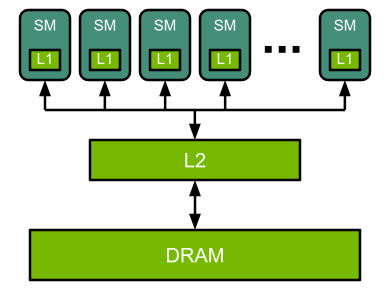
\includegraphics[width=0.70\textwidth]{simple-gpu-arch.png}
	\caption{Memory Hierarchy of the GPU \cite{fig:gpu-arch}}
\end{figure}

Please note that the VRAM is not part of the memory hierarchy, but is
connected to the L2 cache. Caches are used to store frequently used
data and to reduce access times to the main memory. While every SM
has its own L1 cache, the L2 cache is shared between all SMs. Which
means that all cores in one SM are sharing one L1 cache. The CPU
on the other hand has one cache and one memory controller per
core. \cite{CUDA_Programming_Guide}

\section {Summary}

Okay that was a lot of information, so let's summarize the really
important bits what we have learned so far.

The GPU was created to process graphical data much faster than a CPU
could ever do. It allows us to execute the same command on multiple
data simultaneously to prevent waiting for a single command to finish,
which helps us render reoccurring tasks like drawing a texture or model
much faster.  It is made up of many cores which are combined into an
array of streaming multiprocessors (SM) to allow better control and
management of the cores.  The VRAM is the memory of the GPU and its
important to optimize your data to prevent overloading the VRAM.

\chapter{Graphics Rendering Pipeline}

\section{What is the Graphics Pipeline?}

When we talk about the graphics pipeline, I want to make clear that we
are not talking about a physical pipeline that is used to transport data
from one place to another. I've made that mistake when I first started
working with pipelines. My first thought was that the pipeline is a tool
to transport data from the CPU to the GPU, but that's totally wrong.

What is it then? Let's start with a simple definition.

The graphics pipeline is an abstraction layer that is located on the
GPU and is used to process incoming data to create the image that we see
on our screen. \cite{vkGuide} This saves us from writing low level code
explicitly targeting the GPU, which would be a massive task to do.

Please note that the pipeline is implemented differently in every graphics
API, but the basic ideas stay the same. We feed the pipeline with some
graphical data, which then performs operations to transform the data into
an 2D image that can be displayed on our screen. The processed data
is then stored in a so called framebuffer, which I will explain later.
\cite{vkGuide}

There is actually other pipeline types, like the compute or raytracing
pipeline, made for different tasks, but we will focus on the graphics
pipeline for now.

The graphics pipeline is invoked by a draw command,
while the compute pipeline is invoked by a dispatch
command. \cite{build-pipeline} \\
\cite{vulkan-tutorial-compute-shader}

\section{The Basics}

To understand the graphics pipeline, we first need to understand the
how the 2D image on our screen is created from the 3D data that we
provide to the pipeline.

\begin{figure}[hbtp]
	\centering 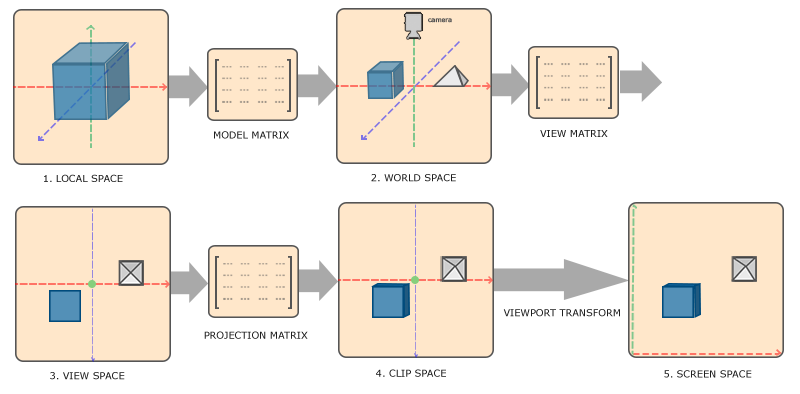
\includegraphics[width=\textwidth]{coordinate-systems.png}
	\caption{Coordinate Systems \cite{fig:view-frustum}}
\end{figure}
\FloatBarrier

We start with the world space, which is the 3D space that we use to
define the positions of our objects in the scene. The world space is
then transformed into the view space, which is the space that the
camera sees. \cite{fig:view-frustum}

But wait, camera? If you have worked with 3D graphics before, you know
that we need a camera that is used to define the space we can view, aka
the view space. The camera is an object that has a view frustum
with a near and far plane, that is used to define what we can see.

\begin{figure}[hbtp]
	\centering 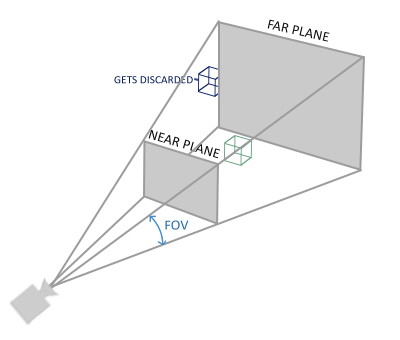
\includegraphics[width=0.60\textwidth]{view-frustum.png}
	\caption{View Frustum \cite{fig:view-frustum}}
\end{figure}
\FloatBarrier

To transform the world space into the view space, we use a view matrix.
Let's briefly talk about matrix transformations and how multiplication
can be used to move, rotate or scale objects in 3D space.

If you have never touched linear algebra before, I suggest you to go over
2Blue1Brown's Essence of Linear Algebra series on YouTube. It is a great
introduction to linear algebra and will help you understand the further topics.

\subsection{Homogeneous Coordinates}

When we want to transform a 3D point, we can use a 4x4 matrix to
transform the point. But why a 4x4 matrix? Because we need to add a
fourth coordinate to the point, which is called the w coordinate. This
coordinate will be used to add perspective to the point, so
that the point or object will appear smaller when it is further away
from the camera. It achieves this by dividing the x, y and z coordinates
by the w coordinate.

\subsection{Matrix Transformations}

When we have an box in 3D space, we can represent its position as an
array of 4 floats, which are the x, y, z and w coordinates of its center.
To move the box, we need to add or subtract a value from the x, y or
z coordinate but how can we do that? We can multiply our position with a translation matrix to
move the box. Wait how do we multiply matrices? It's simple. We multiply
the rows of the first matrix with the columns of the second matrix and add them
together. The result is the value of the new matrix at the position where the row and
column intersect.
\[
	\begin{bmatrix}
		a & b & c \\
		d & e & f \\
		g & h & i \\
	\end{bmatrix}
	x
	\begin{bmatrix}
		j & k & l \\
		m & n & o \\
		p & q & r \\
	\end{bmatrix}
	=
	\begin{bmatrix}
		(aj + bm + cp) & (ak + bn + cq) & (al + bo + cr) \\
		(dj + em + fp) & (dk + en + fq) & (dl + eo + fr) \\
		(gj + hm + ip) & (gk + hn + iq) & (gl + ho + ir) \\
	\end{bmatrix}
\]

\begin{figure}[hbtp]
	\centering \includesvg[width=0.60\textwidth]{images/matrix-multiplication.svg}
	\caption{Matrix Multiplication \cite{fig:matrix-multiplication}}
\end{figure}
\FloatBarrier

Therefor we can create a translation that moves the box by \{tx, ty, tz\}

\[
	\begin{bmatrix}
		1 & 0 & 0 & tx \\
		0 & 1 & 0 & ty \\
		0 & 0 & 1 & tz \\
		0 & 0 & 0 & 1  \\
	\end{bmatrix}
	x
	\begin{bmatrix}
		x \\
		y \\
		z \\
		w \\
	\end{bmatrix}
	=
	\begin{bmatrix}
		x + tx*w \\
		y + ty*w \\
		z + tz*w \\
		w        \\
	\end{bmatrix}
\]

Please note that the w coordinate is changing the x, y and z coordinates,
to adjust the movement to the perspective of the camera.

But what if we want to rotate the box? We can't just add or
subtract a value from the boxes center to rotate it. We need to tackle each
corner of the box and move it around the center of the box.

To rotate the box, we can multiply the position of each corner with a
rotation matrix.

We can use this knowledge to create a rotation matrix. Lets say we have a line with
the points \{0, 0, 0\} and \{1, 0, 0\}.
When we want to rotate this line around an axis by \(\delta\) degrees, we can apply
the following rotation matrices to the points:

x-axis: \[
	\begin{bmatrix}
		1 & 0            & 0           & 0 \\
		0 & cos(\delta)  & sin(\delta) & 0 \\
		0 & -sin(\delta) & cos(\delta) & 0 \\
		0 & 0            & 0           & 1 \\
	\end{bmatrix}
\]

y-axis: \[
	\begin{bmatrix}
		cos(\delta) & 0 & -sin(\delta) & 0 \\
		0           & 1 & 0            & 0 \\
		sin(\delta) & 0 & cos(\delta)  & 0 \\
		0           & 0 & 0            & 1 \\
	\end{bmatrix}
\]

z-axis: \[
	\begin{bmatrix}
		cos(\delta)  & sin(\delta) & 0 & 0 \\
		-sin(\delta) & cos(\delta) & 0 & 0 \\
		0            & 0           & 1 & 0 \\
		0            & 0           & 0 & 1 \\
	\end{bmatrix}
\]

Let's rotate the line around the y axis:

\[
	\begin{bmatrix}
		cos(\delta) & 0 & -sin(\delta) & 0 \\
		0           & 1 & 0            & 0 \\
		sin(\delta) & 0 & cos(\delta)  & 0 \\
		0           & 0 & 0            & 1 \\
	\end{bmatrix}
	\begin{bmatrix}
		0 \\
		0 \\
		0 \\
		1 \\
	\end{bmatrix}
	=
	\begin{bmatrix}
		0 \\
		0 \\
		0 \\
		1 \\
	\end{bmatrix}
\]

\[
	\begin{bmatrix}
		cos(\delta) & 0 & -sin(\delta) & 0 \\
		0           & 1 & 0            & 0 \\
		sin(\delta) & 0 & cos(\delta)  & 0 \\
		0           & 0 & 0            & 1 \\
	\end{bmatrix}
	\begin{bmatrix}
		1 \\
		0 \\
		0 \\
		1 \\
	\end{bmatrix}
	=
	\begin{bmatrix}
		cos(\delta) \\
		0           \\
		sin(\delta) \\
		1           \\
	\end{bmatrix}
\]

You can see that the origin of the line stays the same, but the direction
of the line has changed. This is because we actually rotate the entire
world space and not the object itself. But because the object is in the
world space, it will also be rotated.

Scaling of an object is a bit simpler than rotation. We just multiply
the position of the object with a scaling matrix that
looks like this:

\[
	\begin{bmatrix}
		x & 0 & 0 & 0 \\
		0 & y & 0 & 0 \\
		0 & 0 & z & 0 \\
		0 & 0 & 0 & 1 \\
	\end{bmatrix}
\]

You might see that we simply multiply the x, y and z coordinates with the
scaling factor we want to apply to that axis. So when we want to scale an
object by 2 on the x axis, we would multiply the x coordinate with 2 and
leave the y and z coordinates as they are.

\subsection{View Space}

Now that we know how to transform the world space, we can move the camera
and the objects, so that the camera is the origin of the view space.

To do so we simply take the position of the camera, for example \{1, 2, 3, 1\},
and subtract it from every object in the world space. This will move the
camera to the origin of the view space and keep the objects in the same
position relative to the camera.

\[
	\begin{bmatrix}
		1 & 0 & 0 & -1 \\
		0 & 1 & 0 & -2 \\
		0 & 0 & 1 & -3 \\
		0 & 0 & 0 & 1  \\
	\end{bmatrix}
	\begin{bmatrix}
		x \\
		y \\
		z \\
		w \\
	\end{bmatrix}
	=
	\begin{bmatrix}
		x - 1*w \\
		y - 2*w \\
		z - 3*w \\
		w       \\
	\end{bmatrix}
\]

Looking at the result, we can see that it doesn't really make sense to keep
the w coordinate for the camera, because the camera is not a 3D object.
Therefor we can set the w coordinate of the camera to 1. This will make the homogeneous
coordinates of the camera \{x, y, z, 1\} equal to \{x, y, z\} in 3D space.

Now that the camera is the origin of the view space, we need to rotate everything,
so that the camera is looking down the z axis. Lets say we have a camera that is
is looking down this direction: \{x,y,z\}. We can create a rotation matrix that
rotates the world space so that the camera is looking down the z axis \{0, 0, z\}.

But first we need to get the angles of the rotation. We can do this by using the
dot product of the camera direction and the z axis. The dot product is simply the
cosine of the angle between two vectors. So when we have two vectors \{x, y, z\}
and \{0, 0, z\}, we can calculate the angle between them by using the dot product.

The dot product looks like this:
\[a \cdot b = |a| * |b| * cos(\theta)\]
\[a \cdot b = a_x * b_x + a_y * b_y + a_z * b_z\]

From here we can divide everything by \(|a| * |b|\) to get \(cos(\theta)= \frac{a \cdot b}{|a| * |b|}\).
Let's calculate the angles we need to rotate the camera to look down the z axis.

We start off by rotating the camera, so that it is looking down the xz plane.
This means that the y coordinate of the camera direction is 0. By taking the dot
product of the camera direction and the x axis on the same hight, we can calculate the angle
we need to rotate the camera around the z axis.

\[
	\begin{bmatrix}
		x \\
		y \\
	\end{bmatrix}
	\cdot
	\begin{bmatrix}
		1 \\
		0 \\
	\end{bmatrix}
	=
	\frac{x}{\sqrt{x^2 + y^2}}
	=
	cos(\theta)
\]

Now we just need to rotate the xz plane around the y axis, so that the camera is looking
up the z axis. We can calculate the angle by taking the dot product of the camera direction
after rotating it around the z axis and the z axis itself

\[
	\begin{bmatrix}
		x \\
		z \\
	\end{bmatrix}
	\cdot
	\begin{bmatrix}
		0 \\
		1 \\
	\end{bmatrix}
	=
	\frac{z}{\sqrt{x^2 + z^2}}
	=
	cos(\theta)
\]

Let's calculate the angles for the camera direction \{1, 1, 1\}.

\[
	\theta_z = cos^{-1}(\frac{1}{\sqrt{1^2 + 1^2}})
	=
	cos^{-1}(\frac{1}{\sqrt{2}})
	=
	45\degree
\]

Now that we have the z angle, we can rotate everything by 45 degrees around the z axis.

\[
	\begin{bmatrix}
		cos(\theta_z)  & sin(\theta_z) & 0  & 0 \\
		-sin(\theta_z) & cos(\theta_z) & -1 & 0 \\
		0              & 0             & 1  & 0 \\
		0              & 0             & 0  & 1 \\
	\end{bmatrix}
	\cdot
	\begin{bmatrix}
		1 \\
		1 \\
		1 \\
		1 \\
	\end{bmatrix}
	=
	\begin{bmatrix}
		\sqrt{2} \\
		0        \\
		1        \\
		1        \\
	\end{bmatrix}
\]

Now we calculate the angle for the y axis.

\[
	\theta_y = cos^{-1}(\frac{1}{\sqrt{\sqrt{2}^2 + 1^2}})
	=
	cos^{-1}(\frac{1}{\sqrt{3}})
	=
	54.7\degree
\]

\[
	\begin{bmatrix}
		cos(\theta_y) & 0 & -sin(\theta_y) & 0 \\
		0             & 1 & 0              & 0 \\
		sin(\theta_y) & 0 & cos(\theta_y)  & 0 \\
		0             & 0 & 0              & 1 \\
	\end{bmatrix}
	\cdot
	\begin{bmatrix}
		\sqrt{2} \\
		0        \\
		1        \\
		1        \\
	\end{bmatrix}
	=
	\begin{bmatrix}
		0        \\
		0        \\
		\sqrt{3} \\
		1        \\
	\end{bmatrix}
\]

Don't forget to perform all of this for every object in the world space.
The result will be the view space, where the camera is the origin and
the objects are rotated so that the camera is looking down the z axis.

\subsection{Projection Transformation}

The next step is the transformation from the view space to the canonical
view volume (CVV). The CVV is a that is used to define what we can see
on the screen. It is also called the clip space, because it is used to
clip everything that is outside of the view frustum.

\begin{figure}[hbtp]
	\centering 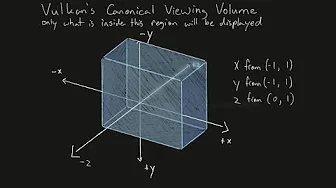
\includegraphics[width=0.80\textwidth]{cvv.png}
	\caption{Canonical View Volume \cite{fig:cvv}}
\end{figure} \FloatBarrier

This task involves transforming the view frustum into a orthographic view
volume, which is a cube with the size of the near plane and the same depth
as the frustum. Then we move the orthographic view volume to the origin
and scale it to the size of the cvv.

Let's start with the transformation of the view frustum to the orthographic
view volume. We basically need to scale the objects so that the far plane is
the same size as the near plane. Normally the near plane is 0.1 units away and the far
plane is 100 units away.

When we're looking at the frustum from the side, we can see that the camera and
the far plane create a triangle that can be divided into two right triangles at the
z axis.

\begin{figure}[hbtp]
	\centering \includesvg[width=0.80\textwidth]{images/perspective.svg}
	\caption{View Frustum}
\end{figure} \FloatBarrier

What we need to calculate is yn, which is the new height of the object.
To do so we use the green triangle and the near planes distance on the z axis
(n) to get the following formula:

\[
	\frac{yn}{n} = \frac{y}{z}
\]

We can use this because the triangles sin angle is the same in the green triangle.
When we solve this for yn, we get:

\[
	yn = \frac{y * n}{z}
\]

The same can be applied for the x axis:

\[
	xn = \frac{x * n}{z}
\]

The z axis stays the same.

So when we have a point \{x, y, z\} in the view space, we need to transform it to \\
\(\{\frac{x * n}{z}, \frac{y * n}{z}, z\}\) to get the orthographic view volume. Unfortunately
there is no way we can divide the x and y value with z with just 3 dimensions. We need to add a 4th coordinate to the point to be able to
divide by z. This is called the perspective divide.

To do so we add a homogeneous variable to the point and transfer the z coordinate to this new w
variable. This will allow us to divide the x, y and z coordinate by the z coordinate.
So what we want is to transform the point \{x, y, z, w\} to \(\{x * n, y * n, z^2, z\}\).
Keep in mind that the homogeneous coordinate is the same as the 3D coordinate after dividing by w.

Okay so what we need is a 4x4 matrix that multiplies the x and y coordinate with n and the z coordinate with itself.
We also need to multiply the w coordinate with z, to move the z coordinate to the w coordinate. This works because
w is like a scaling factor for the x, y and z coordinate but is often set to 1.

\[
	\begin{bmatrix}
		n & 0 & 0   & 0   \\
		0 & n & 0   & 0   \\
		0 & 0 & m_1 & m_2 \\
		0 & 0 & 1   & 0   \\
	\end{bmatrix}
	\begin{bmatrix}
		x \\
		y \\
		z \\
		w \\
	\end{bmatrix}
	=
	\begin{bmatrix}
		x * n \\
		y * n \\
		z^2   \\
		z     \\
	\end{bmatrix}
\]

Okay we have one last problem. How do we get to \(z^2\) ?
First we have the equation \(z^2 = m_1 * z + m_2\), considering w is 1.
The problem is that there are 2 possible solutions for m1 and m2, which we
can not work with. So we need to add 2 constrains to the equation.
We can just say that we want to apply this equation to the near and far planes z coordinate.
So we will say z = n and z = f. This will give us 2 equations that we can solve for m1 and m2.

\[
	\begin{bmatrix}
		n^2 \\
		f^2 \\
	\end{bmatrix}
	=
	\begin{bmatrix}
		m_1 * n + m_2 \\
		m_1 * f + m_2 \\
	\end{bmatrix}
\]

With this we can now calculate m1 and m2.

\( n^2 = m_1 * n + m_2 \) \\
\( m_2 = n^2 - m_1 * n \) \\
\( f^2 = m_1 * f + m_2 \) \\
\( f^2 = m_1 * f + n^2 - m_1 * n \) \\
\( f^2 - n^2 = m_1 * f - m_1 * n \) \\
\( f^2 - n^2 = m_1 * (f - n) \) \\
\( m_1 = \frac{f^2 - n^2}{f - n} \) \\
\( m_1 = f + n \) \\
\( m_2 = n^2 - (f + n) * n \) \\
\( m_2 = n^2 - f * n - n^2 \) \\
\( m_2 = -f * n \) \\

Therefor the final matrix looks like this:

\[
	\begin{bmatrix}
		n & 0 & 0     & 0      \\
		0 & n & 0     & 0      \\
		0 & 0 & f + n & -f * n \\
		0 & 0 & 1     & 0      \\
	\end{bmatrix}
\]

This matrix will actually only give us \(z^2\) on the near and far plane. The Objects in between will have
a little offset on the z axis but will remain linearly interpolated between the near and far plane.

Now that we have the orthographic view volume, we need to move it to the origin and scale it to the size of the CVV.
The CVV looks like this from the front:

\begin{figure}[hbtp]
	\centering \includesvg[width=0.60\textwidth]{images/clip-space.svg}
	\caption{Canonical View Volume Front}
\end{figure} \FloatBarrier

It is a coordinate system where the y axis is flipped and therefore the positive of the z axis is pointing away from us.
Each axis ranges from -1 to 1 except the z axis, which ranges from 0 to 1. This is because the everything negative on the z axis
is behind us and therefor not visible.

Lets first move the orthographic view volumes near planes center to the origin.

\[
	\begin{bmatrix}
		1 & 0 & 0 & -c_x \\
		0 & 1 & 0 & -c_y \\
		0 & 0 & 1 & -c_z \\
		0 & 0 & 0 & 1    \\
	\end{bmatrix}
\]


When the near plane is 0.1 units away, we need to move the orthographic view volume by 0.1 units on the z axis.
So the \(c_z\) value is the distance of the near plane on the z axis aka n.

For the x and y value we just have to calculate the center of the near plane. This is done by adding the opposite
sides together and then dividing them by 2. So for \(c_x\) we get \(\frac{l + r}{2}\) and for \(c_y\) we get \(\frac{t + b}{2}\).

Next we scale the orthographic view volume to the size of the CVV. This is done by multiplying the x, y and z coordinate
with the dimension of the canonical view volume over the size of the orthographic view volume.
We can get the size from subtracting the right side from the left side for the x axis,
the top from the bottom for the y axis and the far from the near plane for the z axis. So the scaling matrix looks like this:

\[
	\begin{bmatrix}
		\frac{2}{r - l} & 0               & 0               & 0 \\
		0               & \frac{2}{t - b} & 0               & 0 \\
		0               & 0               & \frac{1}{f - n} & 0 \\
		0               & 0               & 0               & 1 \\
	\end{bmatrix}
\]

Now we can combine both transformations to get the final projection matrix:

\[
	\begin{bmatrix}
		1 & 0 & 0 & -\frac{l + r}{2} \\
		0 & 1 & 0 & -\frac{t + b}{2} \\
		0 & 0 & 1 & -n               \\
		0 & 0 & 0 & 1                \\
	\end{bmatrix}
	\cdot
	\begin{bmatrix}
		\frac{2}{r - l} & 0               & 0               & 0 \\
		0               & \frac{2}{t - b} & 0               & 0 \\
		0               & 0               & \frac{1}{f - n} & 0 \\
		0               & 0               & 0               & 1 \\
	\end{bmatrix}
	=
	\begin{bmatrix}
		\frac{2}{r - l} & 0               & 0               & -\frac{l + r}{r - l} \\
		0               & \frac{2}{t - b} & 0               & -\frac{t + b}{b - t} \\
		0               & 0               & \frac{1}{f - n} & -\frac{n}{f - n}     \\
		0               & 0               & 0               & 1                    \\
	\end{bmatrix}
\]

This is the projection matrix that is used to transform the view space to the clip space. The clip space is then used to
determine what is visible on the screen and what is not. Everything that is visible will now be projected onto the 2D screen.

But wait, we still have that pesky w coordinate. Luckily Vulkan does the perspective divide for us, so we don't have to worry about it.
After the perspective divide we get the normalized device coordinates (NDC).

\subsection{Viewport Transformation}

The viewport is the area on the screen where the image is displayed. It is defined by the x and y position, the width and height and the
min and max depth and starts at the top left corner of the screen. The viewport transformation is used to transform the NDC to the screen space.
This is done by scaling the x and y coordinate to the width and height of the viewport,
scaling and moving the z coordinate to the depth range and then adding
half of the width to the x coordinate and subtracting half of the height from the y coordinate
to move the origin to the top left corner of the screen.

\[
	\begin{bmatrix}
		\frac{width}{2} & 0                & 0                   & \frac{width}{2}  \\
		0               & \frac{height}{2} & 0                   & \frac{height}{2} \\
		0               & 0                & maxDepth - minDepth & minDepth         \\
		0               & 0                & 0                   & 1                \\
	\end{bmatrix}
\]

This will transform the NDC to the screen space, but we can also add an x and y offset to the viewport to move the image around on the screen.
That would mean we need to add the x and y offset when moving the origin to the top left corner of the screen.

\[
	\begin{bmatrix}
		\frac{width}{2} & 0                & 0                   & \frac{width}{2} + x  \\
		0               & \frac{height}{2} & 0                   & \frac{height}{2} + y \\
		0               & 0                & maxDepth - minDepth & minDepth             \\
		0               & 0                & 0                   & 1                    \\
	\end{bmatrix}
\]

Wow that was a lot of complicated math, but it's important to understand how the world is
projected onto our screen. That's the whole point of 3D graphics after all :P

Don't worry tho if you don't quite understand everything, maybe dive into some other resources to further
understand this topic and until then, do what programmers do best. Copy and paste it from somewhere else.

\section{Stages of the Pipeline}

The Vulkan pipeline consists of multiple stages. Some of them are fixed
and can not be changed, while others are programmable to act as we
want them to. These changeable stages are called shaders and are usually
written in the OpenGL Shading Language (GLSL). These shaders have to be
given to the pipeline as compiled SPIR-V bytecode. \cite{spirv}

Lets take a look at the Vulkan pipeline and its stages:

\begin{figure}[hbtp]
	\centering 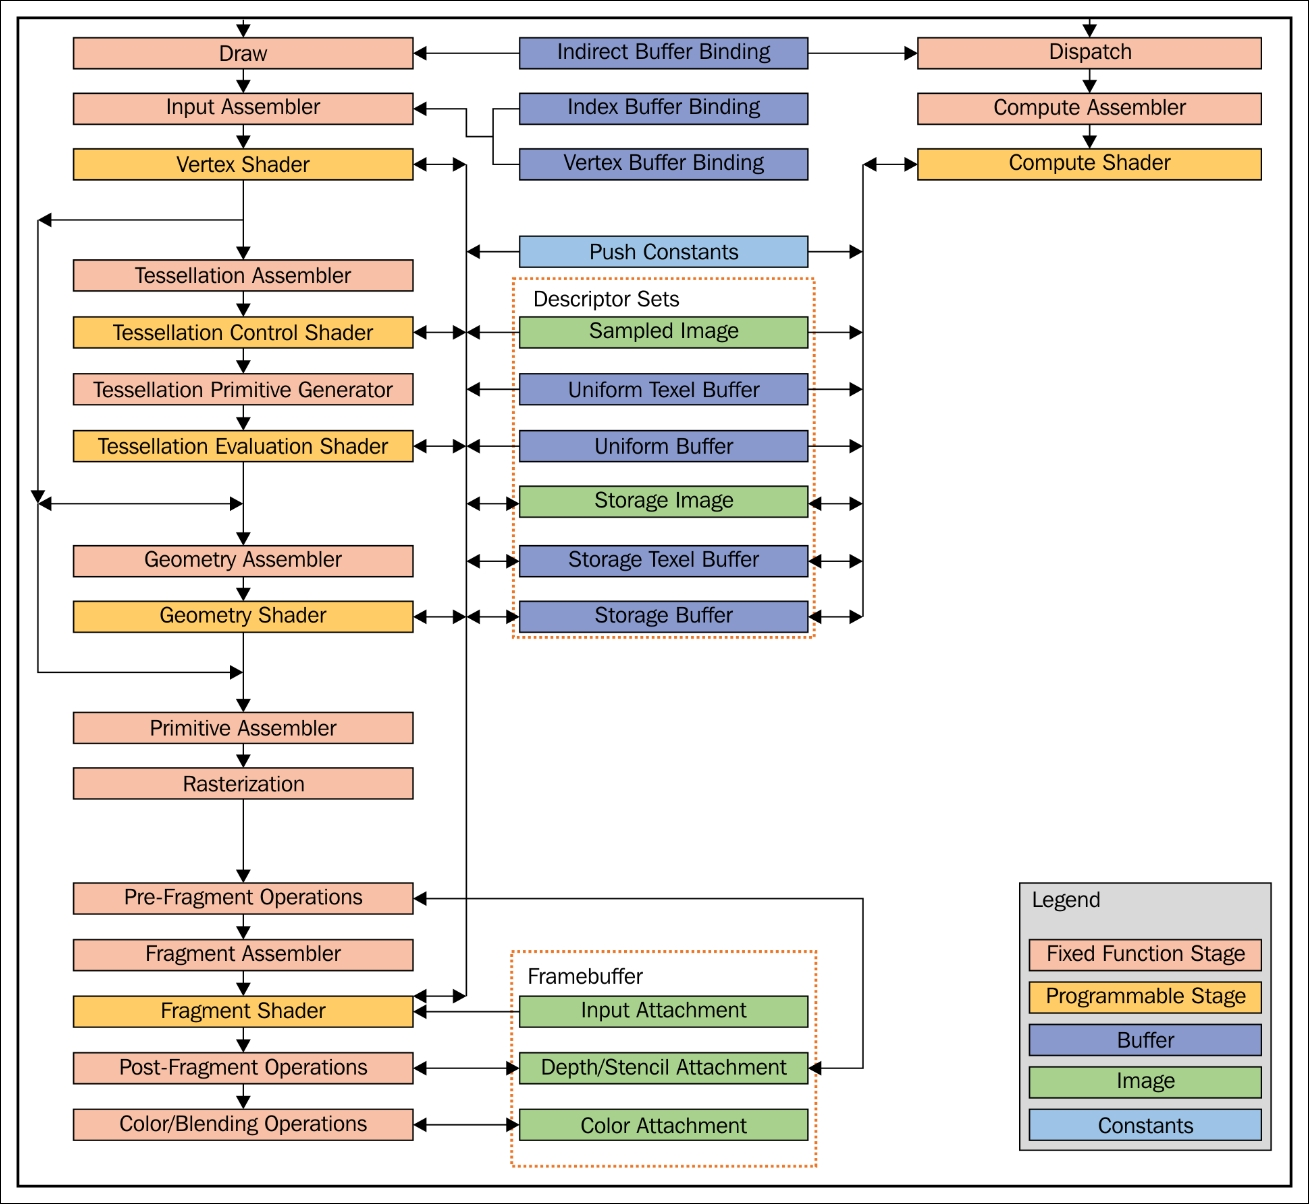
\includegraphics{pipeline.jpg} \caption{Pipeline
		Structure \cite{fig:pipeline}}
\end{figure}

Okay okay, I know that's a lot and there is stuff I haven't talked about
yet, like these Buffers, Images and the Push Constants. Don't worry I
will explain all of these things when going over the stages.

On the left side we have the graphics pipeline and on the right side the
compute pipeline. Now it makes sense that there are different pipelines
for different tasks, right? If we would use the graphics pipeline but
actually just need one shader to edit some data, we would waste a lot
of resources and time sending it though the graphics pipeline.

I'm going to focus on the graphics pipeline and its most important stages.
So some stages will be cut short to better explain the important ones.
In the end you will rarely need to use geometry shaders or tessellation
shaders, but it is important to know that they exist and what they do.

\subsection{Draw}

The draw "stage" is not really a stage, but the command that starts
the rendering process. When we call the vkCmdDraw Command on the GPU,
the pipeline will start processing the data that we have given to
it. \cite{vulkan-spec-draw}

\subsection{Input Assembler}

The input assembler is the first stage of the graphics pipeline. It takes
a vertex and index buffer. \cite{vulkan-spec-pipelines} Before we talk
about the input assembler, lets define what a vertex, index and buffer is.

Basically every model that we see is made up of triangles, and vertices
are the corners of these triangles. A single vertex can contain multiple
attributes like position \{x, y, z\}, color \{r, g, b, a\} or texture
coordinates \{u, v\}. \cite{vulkan-vertex-input}

\begin{figure}[hbtp]
	\centering \includesvg[width=0.60\textwidth]{vektor_triangle.svg}
	\caption{Triangle with vertices}
\end{figure} \FloatBarrier

When we want to reuse certain vertices, for example when
drawing a quad, we can add indices.  These indices tell the
input assembler what vertices need to be combined to form a
triangle. \cite{vulkan-tutorial-index-buffer}

For example: A quad has 4 vertices because it has 4 corners. When we want
to draw the quad we have to create two triangles, which means we need 2 *
3 indices.

Vertices: \{0, 1, 2, 3\} Indices: \{\textcolor{red}{0, 1, 2} ,
\textcolor{blue}{0, 2, 3}\}

\begin{figure}[hbtp]
	\centering \includesvg[width=0.50\textwidth]{vi_quad.svg}
	\caption{Quad
		with vertices created using indices}
\end{figure} \FloatBarrier

Here you can see that the first triangle is created by using the vertices
\{\textcolor{red}{0, 1, 2}\} and the second triangle is created by using
the vertices \{\textcolor{blue}{0, 2, 3}\}. I've added the colors just
to clarify which indices are used to create which triangles.

Now that we know what vertices and indices are, we can talk about how we
provide the GPU with this data. There the buffers come into play. A buffer
is basically an array of data that can be bind to the graphics Pipeline.
When the pipeline is created, we need to provide it with the layout of the
buffer, which tells the pipeline how the data in the buffer is structured.
\cite{vulkan-tutorial-vertex-buffer}

In the Vertex Buffer we store the attributes of each vertex as an
array. An attribute can be a position, color or any other related data
of the Vertex. \cite{vulkan-tutorial-vertex-buffer}

\begin{figure}[hbtp]
	\centering \includesvg[width=1\textwidth]{Vertexbuffer.svg}
	\caption{Interleaved Vertex Buffer}
\end{figure} \FloatBarrier

You can see that each attribute has a specific location in the buffer.
These locations tell the pipeline what bytes belong together. So when
accessing the buffers 0st location it gets an vec3(x,y,z).  The pipeline
also needs to know by what offset, in bytes, each vertex is separated.
In this case it would be 24 bytes, because position and color both
contain 3 floats, which are 4 bytes each. \cite{vulkan-tutorial-vertex-buffer}

This example shows a single buffer containing all attributes in
an interleaved pattern, but we can also create one buffer for each
attribute and then attach them into a single vertexbuffer. This is called
a non-interleaved pattern.

\begin{figure}[hbtp]
	\includesvg[width=1\textwidth]{non-int-vertexbuffer.svg}
	\caption{Non-Interleaved Vertex Buffer}
\end{figure} \FloatBarrier

Each attribute has has its own binding, to tell the pipeline what location
is assigned to the data. So the first binding will always be the position
until you get to the next binding, which will be the color in this case.
\cite{vulkan-tutorial-vertex-buffer}

Usually we will use interleaved buffers, but in some cases, when we need
different attributes for different tasks, we can use non-interleaved
buffers.

The Indexbuffer on the other hand is just an simple array of integers.
\cite{vulkan-tutorial-index-buffer}

Okay we can now finally talk about the input assembler. The input
assembler takes the vertices and indices to create primitives types like
points, lines or triangles. \cite{microsoft-ia}

\newpage

\begin{lstlisting}[language=C++] 

// Provided by VK_VERSION_1_0 typedef
enum VkPrimitiveTopology {
  VK_PRIMITIVE_TOPOLOGY_POINT_LIST = 0, VK_PRIMITIVE_TOPOLOGY_LINE_LIST
  = 1, VK_PRIMITIVE_TOPOLOGY_LINE_STRIP =
  2, VK_PRIMITIVE_TOPOLOGY_TRIANGLE_LIST =
  3, VK_PRIMITIVE_TOPOLOGY_TRIANGLE_STRIP =
  4, VK_PRIMITIVE_TOPOLOGY_TRIANGLE_FAN = 5,
  VK_PRIMITIVE_TOPOLOGY_LINE_LIST_WITH_ADJACENCY = 6,
  VK_PRIMITIVE_TOPOLOGY_LINE_STRIP_WITH_ADJACENCY = 7,
  VK_PRIMITIVE_TOPOLOGY_TRIANGLE_LIST_WITH_ADJACENCY = 8,
  VK_PRIMITIVE_TOPOLOGY_TRIANGLE_STRIP_WITH_ADJACENCY = 9,
  VK_PRIMITIVE_TOPOLOGY_PATCH_LIST = 10,
} VkPrimitiveTopology; 
\end{lstlisting} \cite{vulkan-spec-primitive-topology}

These are the primitive topology types that the input assembler can
create in Vulkan.  We have to tell the input assembler what type of
topology we want to create, which is usually a triangle strip or list,
but we can also create points or lines.  The difference between a list
and a strip is simple. A list will create a triangle for every 3 indices,
while a strip will create a triangle for every 3 indices and then use
the last 2 vertices of the last triangle to create the next triangle.
The same idea works with lines. The "with adjacency" types are only
used when accessing the geometry stage. We will rarely use
the adjacency types, so don't worry on understanding them now. \cite{vulkan-spec-primitive-topology}

\subsection{Vertex Shader}

The vertex shader is the first programmable stage of the pipeline. It takes
the vertices and transforms them by scaling, rotating or translating them
into clip coordinates.
These coordinates range from -1 to 1 on the x, y and z axis, with the center
beginning at \{0, 0, 0\}.

\begin{figure}[hbtp]
	\centering \includesvg[width=0.6\textwidth]{images/clip-space.svg}
	\caption{Clip Coordinates in 2D}
\end{figure} \FloatBarrier

Please note, that the y axis is inverted in clip space and that there is a
z coordinate that can go from 0 to 1, with 0 being directly behind the screen
and 1 being the furthest point that will not be clipped off.

The clip spaced is used to determine if a vertex is visible or not, by
checking if the vertex is in between the -1 and 1 range. \cite{vulkan-tutorial-shader-modules}

\printbibliography[
	heading=bibintoc, title={Bibliography}
]

\listoffigures

\end {document}
